\documentclass[10pt,openany]{book}
 
\usepackage{geometry, graphicx, varioref, soul, verbatim, amsmath, calc, caption, wasysym, footmisc, makeidx, ifthen, subfigure, multicol, epstopdf, enumerate, wrapfig, textcomp, multirow, changepage, setspace, lscape, titlesec}
\usepackage[usenames,dvipsnames]{color}  
%\newcommand{\href}[2]{#2} \newcommand{\url}[1]{#1} \newcommand{\urlstyle}[1]{}

\definecolor{oiGA}{rgb}{0,0,0}
\definecolor{oiGB}{rgb}{.5,.5,.5}
\definecolor{oiGC}{rgb}{.85,.85,.85}
%\definecolor{oiB}{rgb}{0.365,0.529,0.631}
\definecolor{oiB}{rgb}{.337,.608,.741}
%\definecolor{oiB}{rgb}{0,0,0}
\definecolor{oiG}{rgb}{.298,.447,.114}
\definecolor{oiY}{rgb}{.957,.863,0}
\definecolor{oiR}{rgb}{.941,.318,.200}
\definecolor{redcards}{rgb}{.941,.318,.200}


\definecolor{rd}{rgb}{.80,.0,.0}
\definecolor{tableHL}{rgb}{.5,.1,.2}
\definecolor{tableHLBlue}{rgb}{.2,.4,.9}
\definecolor{highlight}{rgb}{.5,.1,.2}
\definecolor{highlightO}{rgb}{.1,.3,.8}
\definecolor{highlightT}{rgb}{.6,.3,.1}
\definecolor{ex}{rgb}{.0,.30,.55}
\definecolor{gray}{rgb}{.5,.5,.5}
\definecolor{steelBlue}{rgb}{.3,.4,.8}
\definecolor{excolor}{rgb}{.0,.3,.55}
\definecolor{secolor}{rgb}{.0,.3,.55}
\definecolor{comment}{rgb}{.65,.45,.25}
\definecolor{grayDark}{rgb}{.43,.43,.43}
\definecolor{grayLight}{rgb}{.65,.65,.65}
\definecolor{examplegray}{rgb}{0,0,0} %{.83,.83,.83}
\definecolor{termOColor}{rgb}{.65,.1,.1}



% _____ Online Version _____ %
\usepackage[bookmarksnumbered, colorlinks = false, pdfborder = {0 0 0}, urlcolor = oiGB, colorlinks=true, linkcolor = oiGB, citecolor = oiGB, backref = true]{hyperref}
\newcommand{\versiondate}[0]{March 5th, 2016}

% _____ B&W Print Version _____ %
%\definecolor{oiB}{rgb}{0,0,0}\usepackage[colorlinks=false,pdfborder={0 0 0},urlcolor= black,colorlinks=black,linkcolor=black, citecolor=black,backref=true]{hyperref}

% _____ COLOR PRINT Version _____ %
%\usepackage[colorlinks=false,pdfborder={0 0 0},urlcolor= black,colorlinks=black,linkcolor=black, citecolor=black,backref=true]{hyperref}

\usepackage[style=authortitle-ibid, maxnames=2,natbib=true,sortcites=true,block=space,backend=bibtex]{biblatex}

\makeindex
% 1 Page Parameters
% 2 Special Commands for Editions
% 3 Content Modifications
% 4 Counters and Parameters
% 5 Section Coloring
% 6 Utilities
% 7 
% 8 Figures and Captions
% 9 Examples and Exercises
% 10 Special Boxes



%-------------------------------------------------------------
% 1 Page Parameters
% 1.1 Amazon
\setlength\paperheight{10in}
\setlength\textheight{8.25in}
\setlength\paperwidth{8in}
\setlength\textwidth{5.45in}
\setlength\voffset{-10mm}
% 1.2 Margin Size
% 1.2.1 Slim
%\setlength\hoffset{0.25in}
%\setlength\oddsidemargin{0.25in}
%\setlength\evensidemargin{0in}
% 1.2.2 Medium
\setlength\hoffset{3.7mm}
\setlength\oddsidemargin{3mm}
\setlength\evensidemargin{3mm}
% 1.2.3 Wide
%\setlength\hoffset{-5mm}
%\setlength\oddsidemargin{0.5in}
%\setlength\evensidemargin{0.5in}
% 1.3 PDF Parameters
%\setlength\paperheight{11in}
%\setlength\textheight{8.25in}
%\setlength\paperwidth{8.5in}
%\setlength\textwidth{5.45in}
%\setlength\voffset{-10mm}
%\setlength\oddsidemargin{0.75in}
%\setlength\evensidemargin{0.75in}
% 1.4 Margin Spacing
\setlength{\marginparsep}{5mm}
\setlength{\marginparwidth}{20mm}


% Tablet Version
%\setlength\paperheight{8.82in}\setlength\textheight{8.25in}\setlength\paperwidth{5.7in}\setlength\textwidth{5.45in}\setlength\voffset{-23.5mm}\setlength\hoffset{-27mm}\setlength\oddsidemargin{5mm}\setlength\evensidemargin{5mm}\setlength{\marginparsep}{5mm}\setlength{\marginparwidth}{35mm}




%-------------------------------------------------------------
% 2 Special Commands for Editions
\newcommand{\textA}[1]{#1}



%-------------------------------------------------------------
% 3 Content Modifications
\newcommand{\APVersion}[2]{#2}
\newcommand{\MultipleRegression}[2]{#1}
\newcommand{\MultipleRegressionChapter}[2]{#1}
\newcommand{\SimulationAndRandomization}[1]{#1}
\newcommand{\ANOVASection}[2]{#1}
\newcommand{\GLMSection}[2]{#1}




%-------------------------------------------------------------
% 4 Counters and Parameters
% 4.1 Counters
\newcounter{alwaysOne}
\setcounter{alwaysOne}{1}
\newcounter{alwaysTwo}
\setcounter{alwaysTwo}{2}
\newcounter{alwaysThree}
\setcounter{alwaysThree}{3}
\newcounter{alwaysFour}
\setcounter{alwaysFour}{4}
\newcounter{withinChNum}[chapter]
\setcounter{withinChNum}{0}
\newcounter{eoce}[chapter]
\renewcommand{\theeoce}{\arabic{chapter}.\arabic{eoce}}
\newcounter{eocesolch}
\setcounter{eocesolch}{0}
\newcounter{eocesol}[eocesolch]
% 4.2 Parameters
\newlength{\exampleAboveBar}
\newlength{\exampleBelowBar}
\setlength{\exampleAboveBar}{-3.15mm}
\setlength{\exampleBelowBar}{-1.15mm}
% 4.3 Chapter Declarations
\newcommand\includechapter[2]{
  \setcounter{chapter}{#1}
  \addtocounter{chapter}{-1}
  \normalsize
  \include{#2/TeX/#2}
  \include{#2/TeX/#2_ex}}



%-------------------------------------------------------------
% 5 Section Coloring
% 5.1 Chapter
\titleformat{\chapter}[display]
{\color{oiB}\normalfont\huge\bfseries\raggedright}{\chaptertitlename\
\thechapter}{20pt}{\Huge}
% 5.2 Section
\titleformat{\section}
{\color{oiB}\normalfont\Large\bfseries}
{\color{oiB}\thesection}{1em}{}
% 5.3 Subsection
\titleformat{\subsection}
{\color{oiB}\normalfont\large\bfseries}
{\color{oiB}\thesubsection}{1em}{}


%-------------------------------------------------------------
% 6 Utilities
% 6.1 Helpful Editing Commands
\newcommand\Add[1]{\marginpar[{\Huge\color{oiR}$\bullet$}]{\Huge\color{oiR}$\bullet$}{\color{oiB}#1}}
\newcommand\Cut[1]{\marginpar[{\Huge\color{oiR}$\bullet$}]{\Huge\color{oiR}$\bullet$}{\color{oiGC}#1}}
\newcommand\Comment[1]{\marginpar[{\Huge\color{oiR}$\bullet$}]{\Huge\color{oiR}$\bullet$} {\color{oiG}{[#1]}}}
\newcommand{\note}[1]{\Comment{#1}}
% 6.2 Special Symbols
\newcommand{\degree}{\ensuremath{^\circ}}
% 6.3 Text Commands (Terms, Data, Variable, Response)
\newcommand{\term}[1]{\textbf{#1}\index{#1|textbf}}
\newcommand{\termsub}[2]{\textbf{#1}\index{#2|textbf}}
\newcommand{\termni}[1]{\textbf{#1}}
\newcommand{\hiddenterm}[1]{#1\index{#1|textbf}}
\newcommand{\indexthis}[2]{#1\index{#2}}
\newcommand{\termO}[1]{\textbf{\color{termOColor}#1}}
\newenvironment{data}[1]{\texttt{#1}}{}
\newenvironment{var}[1]{\texttt{#1}}{}
\newenvironment{resp}[1]{\texttt{#1}}{}
\newenvironment{calctext}[1]{{\color{oiB}\texttt{#1}}}{}
\newenvironment{calctextmath}[1]{{\color{oiB}\mathtt{#1}}}{}
\newenvironment{calcbutton}[1]{{\color{oiB}\texttt{#1}}}{}
% 6.4 Highlighting
\newenvironment{highlight}{\textbf}{}
\newcommand{\highlightO}[1]{\textbf{\color{oiB}#1}}
\newcommand{\highlightT}[1]{\emph{\color{oiR}#1}}
% 6.5 Lengths
\setlength{\parindent}{0.3in}
% 6.6 Hyperreferences
\newcommand{\urlwofont}[1]{\urlstyle{same}\url{#1}}
\newcommand{\oiRedirect}[2]{\href{http://www.openintro.org/redirect.php?go=#1&referrer=ahss_pdf}{#2}}
\newcommand{\videohref}[2][4.5mm]{\oiRedirect{#2}{\raisebox{-0.3mm}[0pt]{
\includegraphics[height=#1]{extraTeX/icons/video_camera}}}}
\newcommand{\sectionvideohref}[2][6mm]{\oiRedirect{#2}{\raisebox{-0.5mm}[0pt]{
\includegraphics[height=#1]{extraTeX/icons/video_camera}}}}



%-------------------------------------------------------------
% 7 



%-------------------------------------------------------------
% 8 Figures and Captions
% 8.1 & 8.2 Table & Figure Numbering
% Thanks @Herbert on StackExchange for helping clean up this style code!
% http://tex.stackexchange.com/questions/176978/latex-numbering-in-counters-appears-to-have-changed/177045?noredirect=1#comment409945_177045
\makeatletter
\let\c@table\c@figure
\makeatother
% 8.3 Caption Width
\newlength{\mycaptionwidth}
\setlength{\mycaptionwidth}{0.825\textwidth}
\setlength{\captionwidth}{\mycaptionwidth}




%-------------------------------------------------------------
% 9 Examples and Exercises
% 9.1 Exercises, within the text
% 9.1.1 Exercise Environment
\newcommand{\excolor}[1]{{\color{excolor}#1}}
\newenvironment{exercise}
{
\begin{itemize}\item[\color{oiB}$\bigodot$]\refstepcounter{equation}\noindent\normalsize\textbf{\color{oiB}Guided Practice \theexercise}\hspace{3mm}}
{\normalsize

\addvspace{3mm}
\end{itemize}}
% 9.1.2 Exercise Fine Tuning
\newcommand\theexercise{\thechapter.\arabic{equation}}
% 9.2 Examples
% 9.2.1 Example Environment
\newcommand\theexample{\thechapter.\arabic{equation}}
\newenvironment{example}[1]
{\begin{itemize}
\item[\color{oiB}\Large$\CIRCLE$]\refstepcounter{equation}\noindent\textbf{\color{oiB}Example \theexample}\hspace{0.3cm}#1\vspace{\exampleAboveBar}

{\color{examplegray}\rule{20mm}{0.1mm}}

\vspace{\exampleBelowBar}

\normalsize}{

\end{itemize}
\addvspace{3mm}
}
% 9.3 EOCEs: End of Chapter Exercises
% 9.3.1 Environment
\newenvironment{eoce}[2]
{\refstepcounter{eoce}\noindent\small\textbf{\textcolor{oiB}{\arabic{chapter}.\arabic{eoce}}}\hspace{2mm} #1

\addvspace{3mm}

}
%{\em #2 } $\:$ \\ }
{}
% 9.3.2 EOCE Solutions
\newcommand{\eocesolch}[1]{
\refstepcounter{eocesolch}\noindent\textbf{\color{oiB}\arabic{eocesolch}\hspace{2mm}#1}

\addvspace{2mm}

}
\newcommand{\eocesol}[1]{\refstepcounter{eocesol}\noindent\textbf{\color{oiB}\arabic{eocesolch}.\arabic{eocesol}}\hspace{2mm}{\small#1}\addtocounter{eocesol}{1}

\addvspace{1mm}

}
% 9.3.3 EOCE Utilities
\newcommand{\qt}[1]{\textcolor{oiB}{\textbf{#1.}}}
\newcommand{\qtq}[1]{\textcolor{oiB}{\textbf{#1?}}}
\newcommand{\ec}[1]{\textcolor{oiB}{\footnotesize{~(#1)}}}% 9.3.4 EOCE Roman Parts
\newenvironment{romanparts}{
\begin{enumerate}[I.]
\setlength{\itemsep}{0mm}
}{\end{enumerate}}
% 9.3.5 EOCE Parts
\newenvironment{parts}{
%\vspace{-0.25cm}
\begin{enumerate}[(a)]
\setlength{\itemsep}{0mm}}
{\end{enumerate}}
% 9.3.6 EOCE Subparts
\newenvironment{subparts}{
\begin{enumerate}[i.]
\setlength{\itemsep}{0mm}}
{\end{enumerate}}
% 9.3.7 EOCE hyp environment
\newenvironment{hyp}{
\begin{itemize}
\setlength{\itemsep}{0mm}
}
{\end{itemize}
}
% 9.3.8 cond environment
\newenvironment{cond}{
\begin{enumerate}[1.]
\setlength{\itemsep}{0mm}
}
{\end{enumerate}
}




%-------------------------------------------------------------
% 10 Special Boxes
% 10.1 Term Box
\newcommand\tBoxTitleBuffer{\\[1.5mm]}
\newenvironment{tBoxTitle}[2][\tBoxTitleBuffer]{\textbf{\color{oiB}#2} #1
}{}
\newenvironment{termBox}[1]{
\addvspace{4mm}
\noindent{\color{oiB}\framebox[\textwidth][c]{\framebox[\textwidth-3mm][l]{ \\
	\vspace{0.5cm} \\
	\begin{minipage}[b]{\textwidth-3mm}
		\begin{minipage}[t]{2mm}
			\hspace{2mm}
		\end{minipage}
		\begin{minipage}[b]{\textwidth-10mm}
			\color{black}\ 
			
			#1
			
			\vspace{1.5mm}
		\end{minipage}
	\end{minipage}}}}
}{

\addvspace{1mm}}
% 10.2 Tip Box
\newenvironment{tipBoxTitle}[2][TIP:\ ]{\textbf{\color{oiB}#1#2} \\
}{}
\newenvironment{tipBox}[1]{
\addvspace{4mm}
\noindent{\color{oiB}\framebox[\textwidth][l]{ \\
	\vspace{5mm} \\
	\begin{minipage}[b]{\textwidth-4mm}
		\begin{minipage}[t]{2mm}
			\hspace{2mm}
		\end{minipage}
		\begin{minipage}[b]{\textwidth-8mm}
			\color{black}\ 
			
			#1
			
			\vspace{1.5mm}
		\end{minipage}
	\end{minipage}}}
}{

\addvspace{1mm}}
% 10.3 Caution Box
\newenvironment{caution}[2]{
\addvspace{4mm}
\noindent{\color{oiB}\framebox[\textwidth][l]{ \\
	\vspace{5mm} \\
	\begin{minipage}[b]{\textwidth-4mm}
		\begin{minipage}[t]{2mm}
			\hspace{2mm}
		\end{minipage}
		\begin{minipage}[b]{\textwidth-8mm}
			\textbf{\color{oiB}Caution: #1} \\
			\color{black}#2
		\end{minipage}
	\end{minipage}}}
}{

\addvspace{1mm}}







%
% Tablet Version
\setlength\paperheight{8.82in}
\setlength\textheight{8.25in}
\setlength\paperwidth{5.7in}
\setlength\textwidth{5.45in}
\setlength\voffset{-23.5mm}
\setlength\hoffset{-27mm}
\setlength\oddsidemargin{5mm}
\setlength\evensidemargin{5mm}
\setlength{\marginparsep}{5mm}
\setlength{\marginparwidth}{35mm}



\title{\huge TI-83/84 Guide for Introductory Statistics\vspace{10mm} \\ \Large Includes step-by-step instructions, \\practice exercises, and links to video \\tutorials.  Covers all calculator features \\needed for AP\textregistered{}  Statistics Exam \vspace{10mm} \\ \Large Instructions excerpted from \\ \emph{Advanced High School Statistics}, \\available for FREE at \href{https://www.openintro.org/stat/textbook.php?stat_book=aps}{openintro.org} \vspace{20mm}}
\author{
Leah Dorazio \\
\small\emph{San Francisco University High School} \\
\small\emph{leah@openintro.org}}

\usepackage{geometry}

\usepackage{remreset}

\makeatletter
  \renewcommand \thesection {\@arabic\c@section}
  \@removefromreset{section}{chapter}
\makeatother
\setcounter{tocdepth}{1}


\begin{document}

\maketitle

\chapter*{}
\vfill

\noindent Copyright $\copyright$ 2016 OpenIntro, Inc. \\
Updated: \today. \\

\noindent This guide is available under a Creative Commons license. % Attribution-ShareAlike license. \\
Visit \oiRedirect{openintro.org}{openintro.org} for a free PDF, to download the source files, or for more information about the license. \\

%\noindent Modified versions of this textbook, including reformatted electronic versions, may not be redistributed under a title that suggests association with or endorsement by OpenIntro, e.g. it cannot be titled \emph{OpenIntro Statistics}. %More information on branding restrictions for derivatives is available on the Rights page at~\href{http://www.openintro.org/rights.php}{openintro.org}.

\noindent {\scriptsize AP\textregistered{} is a trademark registered and owned by the College Board, which was not involved in the production of, and does not endorse, this product.}


%_derivative}

\tableofcontents

\chapter*{Summarizing data}
\addcontentsline{toc}{chapter}{ Summarizing data}


\section*{Entering data}
\addcontentsline{toc}{section}{Entering data}

\begin{termBox}{\tBoxTitle[]{\videohref{casio_1_var_stats_and_box_plot} Casio fx-9750GII: Entering data}
\begin{enumerate}
\setlength{\itemsep}{0mm}
\item Navigate to \calctext{STAT} (\calcbutton{MENU} button, then hit the \calcbutton{2} button or select \calctext{STAT}).
\item Optional: use the left or right arrows to select a particular list.
\item Enter each numerical value and hit \calcbutton{EXE}.
\end{enumerate}
}
\end{termBox}

\section*{Calculating summary statistics and drawing a box plot}
\addcontentsline{toc}{section}{Calculating summary statistics and drawing a box plot}

\begin{termBox}{\tBoxTitle[]{\videohref{casio_1_var_stats_and_box_plot} Casio fx-9750GII: Drawing a box plot and 1-variable statistics}
\begin{enumerate}
\setlength{\itemsep}{0mm}
\item Navigate to \calctext{STAT} (\calcbutton{MENU}, then hit \calcbutton{2}) and enter the data into a list.
\item Go to \calctext{GRPH} (\calcbutton{F1}).
\item Next go to \calctext{SET} (\calcbutton{F6}) to set the graphing parameters.
\item To use the 2nd or 3rd graph instead of \calctext{GPH1}, select \calcbutton{F2} or \calcbutton{F3}.
\item Move down to \calctext{Graph Type} and select the $\calctextmath{\triangleright}$ (\calcbutton{F6}) option to see more graphing options, then select \calctext{Box} (\calcbutton{F2}).
\item If \calctext{XList} does not show the list where you entered the data, hit \calctext{LIST} (\calcbutton{F1}) and enter the correct list number.
\item Leave \calctext{Frequency} at \calctext{1}.
\item For \calctext{Outliers}, choose \calctext{On} (\calcbutton{F1}).
\item Hit \calcbutton{EXE} and then choose the graph where you set the parameters \calcbutton{F1} (most common), \calcbutton{F2}, or \calcbutton{F3}.
\item If desired, explore 1-variable statistics by selecting \calctext{1-Var} (\calcbutton{F1}).
\end{enumerate}
}
\end{termBox}


Calculating the summary statistics will return the following information. It will be necessary to hit the down arrow to see all of the summary statistics.

\begin{center}
\begin{tabular}{ll l ll}
$\calctextmath{\bar{\text{x}}}$ & Mean &\quad&
	\calctext{minX} & Minimum \\
$\calctextmath{\Sigma x}$ & Sum of all the data values &&
	$\calctextmath{Q_1}$ & First quartile \\
$\calctextmath{\Sigma x^2}$ & Sum of all the squared data values &&
	\calctext{Med} & Median\\
$\calctextmath{\sigma x}$ & Population standard deviation &&
	\calctext{maxX} & Maximum \\
\calctext{n} & Sample size or \# of data points
\end{tabular}
\end{center}


\section*{Practice exercises}
\addcontentsline{toc}{section}{Practice exercises}

\begin{exercise}Enter the following 10 data points into the first list on a calculator: {5, 8, 1, 19, 3, 1, 11, 18, 20, 5}. Find the summary statistics and make a box plot of the data.
The summary statistics should be $\calctextmath{\bar{x}} = 9.1$, $\calctextmath{Sx} = 7.475$, $\calctextmath{Q1} = 3$, etc. The box plot should be as follows.
\begin{center}
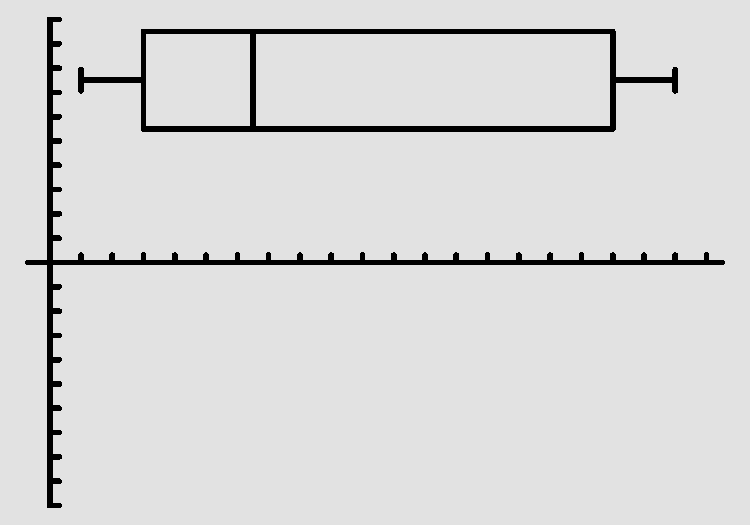
\includegraphics[width=0.45\textwidth]{ch_summarizing_data/figures/TI83_box_plot_A/TI83_box_plot_A}
\end{center}
\end{exercise}


\chapter*{Probability}
\addcontentsline{toc}{chapter}{Probability}

\section*{Computing the binomial coefficient}
\addcontentsline{toc}{section}{Computing the binomial coefficient}

\begin{termBox}{\tBoxTitle[]{\videohref{casio_binomial_coefficient} Casio fx-9750GII: Computing the binomial coefficient, ${n\choose k}$}
\begin{enumerate}
\setlength{\itemsep}{0mm}
\item Navigate to the \calctext{RUN-MAT} section (hit \calcbutton{MENU}, then hit \calcbutton{1}).
\item Enter a value for $n$.
\item Go to \calctext{CATALOG} (hit buttons \calcbutton{SHIFT} and then \calcbutton{7}).
\item Type \calctext{C} (hit the \calcbutton{ln} button), then navigate down to the bolded \calctext{\textbf{C}} and hit \calcbutton{EXE}.
\item Enter the value of $k$. Example of what it should look like: \calctext{7\textbf{C}3}.
\item Hit \calcbutton{EXE}.
\end{enumerate}
}
\end{termBox}



\section*{Binomial calculations}
\addcontentsline{toc}{section}{Binomial calculations}

\begin{termBox}{\tBoxTitle[]{\videohref{casio_binomial_calculations} Casio fx-9750GII: Binomial calculations}
\begin{enumerate}
\setlength{\itemsep}{0mm}
\item Navigate to \calctext{STAT} (\calcbutton{MENU}, then hit \calcbutton{2}).
\item Select \calctext{DIST} (\calcbutton{F5}), and then \calctext{BINM} (\calcbutton{F5}).
\item Choose whether to calculate the binomial distribution for a specific number of successes, $P(X = k)$, or for a range $P(X \leq k)$ of values (0~successes, 1~success, ..., $k$~successes).\vspace{-1.5mm}
  \begin{itemize}
  \setlength{\itemsep}{0mm}
  \item For a specific number of successes, choose \calctext{Bpd} (\calcbutton{F1}). %, which stands for \emph{binomial probability distribution}.
  \item To consider the range 0, 1, ..., $k$ successes, choose \calctext{Bcd}(\calcbutton{F1}). %, which stands for \emph{binomial cumulative distribution}.
  \end{itemize}
\item If needed, set \calctext{Data} to \calctext{Variable} (\calctext{Var} option, which is \calcbutton{F2}).
\item Enter the value for \calctext{x} ($k$), \calctext{Numtrial} ($n$), and \calctext{p} (probability of a success).
\item Hit \calctext{EXE}.
\end{enumerate}
}
\end{termBox}

\section*{Practice exercises}
\addcontentsline{toc}{section}{Practice exercises}

\begin{exercise}
Find the number of ways of arranging 3 blue marbles and 2 red marbles.\footnote{Use $n$ = 5 and $k$ = 3 to get 10.}
\end{exercise}

\begin{exercise}There are 13 marbles in a bag. 4 are blue and 9 are red. Randomly draw 5 marbles \emph{with replacement}. Find the probability you get exactly 3 blue marbles.\footnote{Use $n$ = 5, $p$ = 4/13, and $x$ ($k$) = 3 to get 0.1396.}
\end{exercise}

\begin{exercise}There are 13 marbles in a bag. 4 are blue and 9 are red. Randomly draw 5 marbles \emph{with replacement}. Find the probability you get \emph{at most} 3 blue marbles (i.e. less than or equal to 3 blue marbles).\footnote{Use $n = 5$, $p = 4/13$, and $x = 3$ to get 0.9662.}
\end{exercise}



\chapter*{Distribution of random variables}
\addcontentsline{toc}{chapter}{Distribution of random variables}


\section*{Finding area under the normal curve}
\addcontentsline{toc}{section}{Finding area under the normal curve}


\begin{termBox}{\tBoxTitle[]{\videohref{casio_normal_curve_area} Casio fx-9750GII: Finding area under the normal curve}
\begin{enumerate}
\setlength{\itemsep}{0mm}
\item Navigate to \calctext{STAT} (\calcbutton{MENU}, then hit \calcbutton{2}).
\item Select \calctext{DIST} (\calcbutton{F5}), then \calctext{NORM} (\calcbutton{F1}), and then \calctext{Ncd} (\calcbutton{F2}).
\item If needed, set \calctext{Data} to \calctext{Variable} (\calctext{Var} option, which is \calcbutton{F2}).
\item Enter the \calctext{Lower} Z-score and the \calctext{Upper} Z-score. Set $\calctextmath{\sigma}$ to \calctext{1} and $\calctextmath{\mu}$ to \calctext{0}.\vspace{-1.5mm}
  \begin{itemize}
  \setlength{\itemsep}{0mm}
  \item If finding just a lower tail area, set \calctext{Lower} to \calctext{-12}.
  \item For an upper tail area, set \calctext{Upper} to \calctext{12}.
  %\item If finding a middle area (e.g. $Z_{lower} = 0.5$ to $Z_{upper} = 1.5$), set the \calctext{lower} and \calctext{upper} values appropriately.
  \end{itemize}
\item Hit \calctext{EXE}, which will return the area probability (\calctext{p}) along with the Z-scores for the lower and upper bounds.
\end{enumerate}
}
\end{termBox}


\section*{Find a Z-score that corresponds to a percentile}
\addcontentsline{toc}{section}{Find a Z-score that corresponds to a percentile}


\begin{termBox}{\tBoxTitle[]{\videohref{casio_Z_score_for_a_percentile} Casio fx-9750GII: Find a Z-score that corresponds to a percentile}
\begin{enumerate}
\setlength{\itemsep}{0mm}
\setlength{\itemsep}{0mm}
\item Navigate to \calctext{STAT} (\calcbutton{MENU}, then hit \calcbutton{2}).
\item Select \calctext{DIST} (\calcbutton{F5}), then \calctext{NORM} (\calcbutton{F1}), and then \calctext{InvN} (\calcbutton{F3}).
\item If needed, set \calctext{Data} to \calctext{Variable} (\calctext{Var} option, which is \calcbutton{F2}).
\item Decide which tail area to use (\calctext{Tail}), the tail area (\calctext{Area}), and then enter the $\calctextmath{\sigma}$ and $\calctextmath{\mu}$ values.
\item Hit \calctext{EXE}.
\end{enumerate}
}
\end{termBox}


\section*{Practice exercises}
\addcontentsline{toc}{section}{Practice exercises}

\begin{example}{Use a calculator to determine what percentile corresponds to a Z-score of 1.5.}
Always first sketch a graph:\footnote{normalcdf gives the result without drawing the graph. To draw the graph, do 2nd VARS, DRAW, 1:ShadeNorm. However, beware of errors caused by other plots that might interfere with this plot.}
\begin{center}
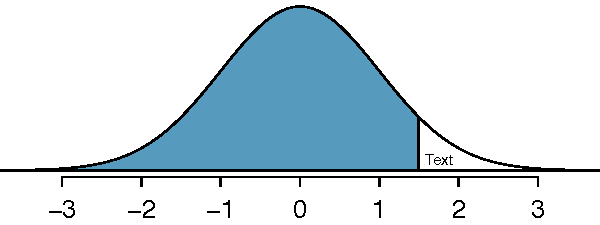
\includegraphics[width=0.57\textwidth]{ch_distributions/figures/zscoreleftof1point5/zscoreleftof1point5}\vspace{-2mm}
\end{center}
To find an area under the normal curve using a calculator, first identify a lower bound and an upper bound. Theoretically, we want all of the area to the left of 1.5, so the left endpoint should be -$\infty$. However, the area under the curve is nearly negligible when $Z$ is smaller than -4, so we will use -5 as the lower bound when not given a lower bound (any other negative number smaller than -5 will also work). Using a lower bound of -5 and an upper bound of 1.5, we get $P(Z < 1.5) = 0.933$.
\end{example}

\begin{exercise}
Find the area under the normal curve to right of $Z=2$.~\footnote{Now we want to shade to the right. Therefore our lower bound will be 2 and the upper bound will be +5 (or a number bigger than 5) to get $P(Z > 2) = 0.023$.}
\end{exercise}

\begin{exercise}Find the area under the normal curve between -1.5 and~1.5.~\footnote{Here we are given both the lower and the upper bound. Lower bound is -1.5 and upper bound is 1.5. The area under the normal curve between -1.5 and 1.5 = $P(-1.5 < Z < 1.5) = 0.866$.}
\end{exercise}


\begin{example}{Use a calculator to find the Z-score that corresponds to the 40th percentile.}Letting Area be 0.40, a calculator gives -0.253. This means that $Z = -0.253$ corresponds to the 40th percentile, that~is, $P(Z < -0.253) = 0.40$.
\end{example}

\begin{exercise}Find the Z-score such that 20 percent of the area is to the right of that Z-score.\footnote{If 20\% of the area is the right, then 80\% of the area is to the left. Letting area be 0.80, we get $Z = 0.841$.}
\end{exercise}	


\chapter*{Inference for categorical data}
\addcontentsline{toc}{chapter}{Inference for categorical data}


\section*{1-proportion $z$-interval and $z$-test}
\addcontentsline{toc}{section}{1-proportion $z$-interval and $z$-test}


\begin{termBox}{\tBoxTitle[]{\videohref{casio_1_prop_inference} Casio fx-9750GII: 1-proportion z-interval}
% Quick navigation: \calctext{STAT} (via \calcbutton{MENU} button), \calctext{INTR}, \calctext{Z}, and \calctext{1-P}.
\begin{enumerate}
\setlength{\itemsep}{0mm}
\item Navigate to \calctext{STAT} (\calcbutton{MENU} button, then hit the \calcbutton{2} button or select \calctext{STAT}).
\item Choose the \calctext{INTR} option (\calcbutton{F4} button).
\item Choose the \calctext{Z} option (\calcbutton{F1} button).
\item Choose the \calctext{1-P} option (\calcbutton{F3} button).
\item Specify the interval details:\vspace{-1.5mm}
  \begin{itemize}
  \setlength{\itemsep}{0mm}
  \item Confidence level of interest for \calctext{C-Level}.
  \item Enter the number of successes, \calctext{x}.
  \item Enter the sample size, \calctext{n}.
  \end{itemize}
\item Hit the \calcbutton{EXE} button, which returns \\[1mm]
  \begin{tabular}{ll}
  \calctext{Left}, \calctext{Right} & ends of the confidence interval \\
  $\calctextmath{\hat{p}}$ & sample proportion \\
  \calctext{n} & sample size
  \end{tabular}
\end{enumerate}
}
\end{termBox}

\newpage


\begin{termBox}{\tBoxTitle{\videohref{casio_1_prop_inference} Casio fx-9750GII: 1-proportion z-test}
%Quick navigation: \calctext{STAT} (via \calcbutton{MENU} button), \calctext{TEST}, \calctext{Z}, and \calctext{1-P}.
The steps closely match those of the 1-proportion confidence interval.
\begin{enumerate}
\setlength{\itemsep}{0mm}
%\item Navigation is nearly the same as for the 1-proportion confidence interval: \\
\item Navigate to \calctext{STAT} (\calcbutton{MENU} button, then hit the \calcbutton{2} button or select \calctext{STAT}).
\item Choose the \calctext{TEST} option (\calcbutton{F3} button).
\item Choose the \calctext{Z} option (\calcbutton{F1} button).
\item Choose the \calctext{1-P} option (\calcbutton{F3} button).
%  navigate to \calctext{STAT} using the \calcbutton{MENU} button,
%  then go to \calctext{TEST} (instead of \calctext{INTR}),
%  choose \calctext{Z}, and
%  then choose \calctext{1-P}.
\item Specify the test details:
  \begin{itemize}
  \setlength{\itemsep}{0mm}
  \item Specify the sidedness of the test using the \calcbutton{F1}, \calcbutton{F2}, and \calcbutton{F3} keys.
  \item Enter the null value, \calctext{p0}.
  \item Enter the number of successes, \calctext{x}.
  \item Enter the sample size, \calctext{n}.
  \end{itemize}
\item Hit the \calcbutton{EXE} button, which returns \\[1mm]
  \begin{tabular}{ll}
  \calctext{z} &  Z-statistic \\
  \calctext{p} &  p-value \\
  $\calctextmath{\hat{p}}$ &  the sample proportion \\
  \calctext{n} &  the sample size
  \end{tabular}
\end{enumerate}
}
\end{termBox}


\section*{Practice exercises}
\addcontentsline{toc}{section}{Practice exercises}

\begin{exercise}
A candidate selects a random sample of size $n=500$.  The proportion of people in the sample that support her is 52\%.  Is there significant evidence that greater than 50\% of the population support her?  Use a calculator to find the p-value for a test with  H$_A: p >$ 50\%.~\footnote{p-value = 0.19}
\end{exercise}

\begin{exercise}
What percent of Americans believe the Supreme Court is doing a good job?  A random sample of  $n = 976$ yields a sample percent of 44\%.  Use a calculator to find a 90\% confidence interval for the percent of all Americans that believe the Supreme Court is doing a good job.~\footnote{The interval is (0.414, 0.471) =  (41.4\%, 47.1\%). }
\end{exercise}

\section*{2-proportion $z$-interval and $z$-test}
\addcontentsline{toc}{section}{2-proportion $z$-interval and $z$-test}


\begin{termBox}{\tBoxTitle[]{\videohref{casio_2_prop_inference} Casio fx-9750GII: 2-proportion z-interval}
\begin{enumerate}
\setlength{\itemsep}{0mm}
\item Navigate to \calctext{STAT} (\calcbutton{MENU} button, then hit the \calcbutton{2} button or select \calctext{STAT}).
\item Choose the \calctext{INTR} option (\calcbutton{F4} button).
\item Choose the \calctext{Z} option (\calcbutton{F1} button).
\item Choose the \calctext{2-P} option (\calcbutton{F4} button).
\item Specify the interval details:
  \begin{itemize}
  \item Confidence level of interest for \calctext{C-Level}.
  \item Enter the number of successes for each group, \calctext{x1} and \calctext{x2}.
  \item Enter the sample size for each group, \calctext{n1} and \calctext{n2}.
  \end{itemize}
\item Hit the \calcbutton{EXE} button, which returns \\[1mm]
  \begin{tabular}{ll}
  \calctext{Left}, \calctext{Right}  &  the ends of the confidence interval \\
  $\calctextmath{\hat{p}1}$, $\calctextmath{\hat{p}2}$ &
  				the sample proportions \\
  \calctext{n1}, \calctext{n2} & sample sizes
  \end{tabular}
\end{enumerate}
}
\end{termBox}

\begin{termBox}{\tBoxTitle[]{\videohref{casio_2_prop_inference} Casio fx-9750GII: 2-proportion z-test}
\begin{enumerate}
\setlength{\itemsep}{0mm}
\item Navigate to \calctext{STAT} (\calcbutton{MENU} button, then hit the \calcbutton{2} button or select \calctext{STAT}).
\item Choose the \calctext{TEST} option (\calcbutton{F3} button).
\item Choose the \calctext{Z} option (\calcbutton{F1} button).
\item Choose the \calctext{2-P} option (\calcbutton{F4} button).
\item Specify the test details:
  \begin{itemize}
  \setlength{\itemsep}{0mm}
  \item Specify the sidedness of the test using the \calcbutton{F1}, \calcbutton{F2}, and \calcbutton{F3} keys.
  \item Enter the number of successes for each group, \calctext{x1} and \calctext{x2}.
  \item Enter the sample size for each group, \calctext{n1} and \calctext{n2}.
  \end{itemize}
\item Hit the \calcbutton{EXE} button, which returns \\[1mm]
  \begin{tabular}{ll ll l}
  \calctext{z} & Z-statistic & \hspace{3mm} &
  	$\calctextmath{\hat{p}1}$, $\calctextmath{\hat{p}2}$ & sample proportions \\
  \calctext{p} & p-value && $\calctextmath{\hat{p}}$ & pooled proportion \\
  &&& \calctext{n1}, \calctext{n2} &  sample sizes
  \end{tabular}
\end{enumerate}}
\end{termBox}


\section*{Practice exercises}
\addcontentsline{toc}{section}{Practice exercises}

\begin{exercise}{Use the data in Table~\ref{24DAndCancerInDogsTableInCalcSection} and a calculator to find a 95\% confidence interval for the difference in proportion of dogs with cancer that have been exposed to 2,4-D versus not exposed to 2,4-D.}\footnote{Correctly going through the calculator steps should lead to an interval of (0.01484, 0.11926). There is no value given for the pooled proportion since we do not pool for confidence intervals.}
\end{exercise}

\begin{table}[h]
\centering
\begin{tabular}{rrr}
  \hline
 & cancer & no cancer \\
  \hline
2,4-D & 191 & 304 \\
no 2,4-D & 300 & 641 \\
   \hline
\end{tabular}
\caption{Summary results for cancer in dogs and the use of 2,4-D by the dog's owner.}
\label{24DAndCancerInDogsTableInCalcSection}
\end{table}


\begin{exercise}{Use the data in Table~\ref{24DAndCancerInDogsTableInCalcSection} and a calculator to find the Z-score and p-value for one-sided test with H$_A$: dogs with cancer are more likely to have been exposed to 2,4-D than dogs without cancer, $p_c - p_n > 0$.}\footnote{Correctly going through the calculator steps should lead to a solution with $Z=2.55$ and $\text{p-value}=0.0055$. The pooled proportion is $\hat{p}=0.342$.}
\end{exercise}

\newpage

\section*{Finding areas under the Chi-square curve}
\addcontentsline{toc}{section}{Finding area unders the Chi-square curve}


\begin{termBox}{\tBoxTitle[]{\videohref{casio_chisq_tail_area} Casio fx-9750GII: Finding an upper tail area under the chi-sq.~curve}
\begin{enumerate}
\setlength{\itemsep}{0mm}
\item Navigate to \calctext{STAT} (\calcbutton{MENU} button, then hit the \calcbutton{2} button or select \calctext{STAT}).
\item Choose the \calctext{DIST} option (\calcbutton{F5} button).
\item Choose the \calctext{CHI} option (\calcbutton{F3} button).
\item Choose the \calctext{Ccd} option (\calcbutton{F2} button).
\item If necessary, select the \calctext{Var} option (\calcbutton{F2} button).
\item Enter the \calctext{Lower} bound (generally the chi-square value).
\item Enter the \calctext{Upper} bound (use a large number, such as 1000).
\item Enter the degrees of freedom, \calctext{df}.
\item Hit the \calcbutton{EXE} button.
\end{enumerate}
}
\end{termBox}


\section*{Chi-square goodness of fit test}
\addcontentsline{toc}{section}{Chi-square goodness of fit test}


\begin{termBox}{\tBoxTitle[]{\videohref{casio_chisq_GOF_test} Casio fx-9750GII: Chi-square goodness of fit test\vspace{0.5mm}}
\begin{enumerate}
\setlength{\itemsep}{0mm}
\item Navigate to \calctext{STAT} (\calcbutton{MENU} button, then hit the \calcbutton{2} button or select \calctext{STAT}).
\item Enter the observed counts into a list (e.g. \calctext{List 1}) and the expected counts into list (e.g. \calctext{List 2}).
\item Choose the \calctext{TEST} option (\calcbutton{F3} button).
\item Choose the \calctext{CHI} option (\calcbutton{F3} button).
\item Choose the \calctext{GOF} option (\calcbutton{F1} button).
\item Adjust the \calctext{Observed} and \calctext{Expected} lists to the corresponding list numbers from Step~2.
\item Enter the degrees of freedom, \calctext{df}.
\item Specify a list where the contributions to the test statistic will be reported using~\calctext{CNTRB}. This list number should be different from the others.
\item Hit the \calcbutton{EXE} button, which returns \\[1mm]
  \begin{tabular}{l ll}
  $\calctextmath{x^2}$ & chi-square test statistic \\
  \calctext{p} & p-value \\
  \calctext{df} & degrees of freedom \\
  \calctext{CNTRB} & list showing the test statistic contributions
  \end{tabular}
\end{enumerate}
}
\end{termBox}

\section*{Chi-square test for two-way tables}
\addcontentsline{toc}{section}{Chi-square test for two-way tables}


\begin{termBox}{\tBoxTitle[]{\videohref{casio_chisq_2_way_test} Casio fx-9750GII: Chi-square test of homogeneity and independence}
\begin{enumerate}
\setlength{\itemsep}{0mm}
\item Navigate to \calctext{STAT} (\calcbutton{MENU} button, then hit the \calcbutton{2} button or select \calctext{STAT}).
\item Choose the \calctext{TEST} option (\calcbutton{F3} button).
\item Choose the \calctext{CHI} option (\calcbutton{F3} button).
\item Choose the \calctext{2WAY} option (\calcbutton{F2} button).
\item Enter the data into a matrix:
  \begin{itemize}
  \item Hit $\calctextmath{\triangleright}$\calctext{MAT} (\calcbutton{F2} button).
  \item Navigate to a matrix you would like to use (e.g. \calctext{Mat C}) and hit \calcbutton{EXE}.
  \item Specify the matrix dimensions: \calctext{m} is for rows, \calctext{n} is for columns.
  \item Enter the data.
  \item Return to the test page by hitting \calcbutton{EXIT} twice.
  \end{itemize}
\item Enter the \calctext{Observed} matrix that was used by hitting \calctext{MAT} (\calcbutton{F1} button) and the matrix letter (e.g.~\calcbutton{C}).
\item Enter the \calctext{Expected} matrix where the expected values will be stored (e.g.~\calcbutton{D}).
\item Hit the \calcbutton{EXE} button, which returns \\[1mm]
  \begin{tabular}{l ll}
  $\calctextmath{x^2}$ & chi-square test statistic \\
  \calctext{p} & p-value \\
  \calctext{df} & degrees of freedom \\
  \end{tabular}
\item To see the expected values of the matrix, go to $\calctextmath{\triangleright}$\calctext{MAT} (\calcbutton{F6} button) and select the corresponding matrix.
\end{enumerate}
}
\end{termBox}


\newpage 

\section*{Practice exercises}
\addcontentsline{toc}{section}{Practice exercises}

\begin{exercise}
Use a calculator to find the area to right of 5.1 for a chi-square distribution with 5 degrees of freedom, i.e. find the upper tail area using a cutoff of 5.1. ~\footnote{Using $df = 5$ and a \emph{lower} bound of $5.1$ for the tail, the upper tail area is 0.4038.}
\end{exercise}


\begin{exercise}
Use the table below and a calculator to find the $X^2$ statistic, df, and p-value for chi-square goodness of fit test.~\footnote{You should find that $X^2=15.08$, $df=6$, and $\text{p-value}=0.0196$.}
\end{exercise}

\begin{table}[h]
\centering
\begin{tabular}{ll ccc ccc c ll}
\hline
Days	 & \hspace{1mm} & 1 & 2 & 3 & 4 & 5 & 6 & 7+ & \hspace{1mm} & Total \\
\hline
Observed values&		& 1532 & 760 & 338 & 194 & 74 & 33 & 17 & & 2948 \\
Expected values &  & 1569 & 734 & 343 & 161 & 75 & 35 & 31 & & 2948 \\
\hline
\end{tabular}
\caption{Distribution of the waiting time until a positive trading day. The expected counts are based on a geometric model.}
\end{table}


\begin{exercise}
Use the table below and a calculator to find the expected values and the $X^2$ statistic, $df$, and p-value for the corresponding chi-square test.~\footnote{First create a $2\times 3$ matrix ith the data. The final summaries should be $X^2=106.4$, $\text{\mbox{p-value}} = 8.06 \times 10^{-24}\approx 0$, and $df=2$. Below is the matrix of expected values:
\begin{center}
\begin{tabular}{l ccc}
&Obama  &Congr. Dem. & Congr. Rep. \\
\hline
Approve				    & 731.59    & 693.45 & 693.96   \\
Disapprove			    & 726.41    & 688.55 & 689.04  \\
\hline
\end{tabular}
\end{center}
}
\end{exercise}


\begin{table}[h]
\centering
\begin{tabular}{ll ccc ll}
& & & \multicolumn{2}{c}{Congress} & \\
\cline{4-5}
 & \hspace{1mm} & Obama & Democrats & Republicans & \hspace{1mm} & Total \\
\hline
Approve				   & & 842    & 736 & 541   & 				& 2119 \\
Disapprove			   & & 616    & 646 & 842   &				& 2104 \\
\hline
Total					   & & 1458    & 1382 & 1383 & 				& 4223 \\
\hline
\end{tabular}
\caption{Pew Research poll results of a March 2012 poll.}
\end{table}


\chapter*{Inference for numerical data}
\addcontentsline{toc}{chapter}{Inference for numerical data}


\section*{1-sample $t$-test and $t$-interval}
\addcontentsline{toc}{section}{1-sample $t$-test and $t$-interval}


\begin{termBox}{\tBoxTitle[]{\videohref{casio_1_mean_inference} Casio fx-9750GII: 1-sample $t$-test}
\begin{enumerate}
\setlength{\itemsep}{0mm}
\item Navigate to \calctext{STAT} (\calcbutton{MENU} button, then hit the \calcbutton{2} button or select \calctext{STAT}).
\item If necessary, enter the data into a list.
\item Choose the \calctext{TEST} option (\calcbutton{F3} button).
\item Choose the \calctext{t} option (\calcbutton{F2} button).
\item Choose the \calctext{1-S} option (\calcbutton{F1} button).
\item Choose either the \calctext{Var} option (\calcbutton{F2}) or enter the data in using the \calctext{List} option.
\item Specify the test details:
  \begin{itemize}
  \setlength{\itemsep}{0mm}
  \item Specify the sidedness of the test using the \calcbutton{F1}, \calcbutton{F2}, and \calcbutton{F3} keys.
  \item Enter the null value, $\calctextmath{\mu}$\calctext{0}.
  \item If using the \calctext{Var} option, enter the summary statistics. If using \calctext{List}, specify the list and leave \calctext{Freq} values at \calctext{1}.
  \end{itemize}
\item Hit the \calcbutton{EXE} button, which returns \\[1mm]
\begin{tabular}{ll l ll}
& alternative hypothesis &\hspace{5mm}&
	$\calctextmath{\bar{x}}$ & sample mean \\
\calctext{t} & T statistic &&
	\calctext{sx} & sample standard deviation \\
\calctext{p} & p-value &&
	\calctext{n} & sample size
\end{tabular}
\end{enumerate}
}
\end{termBox}

\newpage


\begin{termBox}{\tBoxTitle[]{\videohref{casio_1_mean_inference} Casio fx-9750GII: 1-sample $t$-interval}
\begin{enumerate}
\setlength{\itemsep}{0mm}
\item Navigate to \calctext{STAT} (\calcbutton{MENU} button, then hit the \calcbutton{2} button or select \calctext{STAT}).
\item If necessary, enter the data into a list.
\item Choose the \calctext{INTR} option (\calcbutton{F3} button), \calctext{t} (\calcbutton{F2} button), and \calctext{1-S} (\calcbutton{F1} button).
\item Choose either the \calctext{Var} option (\calcbutton{F2}) or enter the data in using the \calctext{List} option.
\item Specify the interval details:
  \begin{itemize}
  \setlength{\itemsep}{0mm}
  \item Confidence level of interest for \calctext{C-Level}.
  \item If using the \calctext{Var} option, enter the summary statistics. If using \calctext{List}, specify the list and leave \calctext{Freq} value at \calctext{1}.
  \end{itemize}
\item Hit the \calcbutton{EXE} button, which returns \\[1mm]
\begin{tabular}{ll}
  \calctext{Left}, \calctext{Right} & ends of the confidence interval \\
  $\calctextmath{\bar{x}}$ & sample mean \\
  \calctext{sx} & sample standard deviation \\
  \calctext{n} & sample size
\end{tabular}
\end{enumerate}
}
\end{termBox}



\section*{Practice exercises}
\addcontentsline{toc}{section}{Practice exercises}

\begin{exercise}
The average time for all runners who finished the Cherry Blossom Run in 2006 was 93.29 minutes. In 2012, the average time for 100 randomly selected participants was 95.61, with a standard deviation of 15.78 minutes. Use a calculator to find the $T$ statistic and p-value for the appropriate test to see if the average time for the participants in 2012 is different than it was in 2006.\footnote{Let $\mu_0$ be 93.29. Choose $\neq$ to correspond to $H_A$. $T=1.47$, $df = 99$, and p-value$=0.14$.}
\end{exercise}

\begin{exercise}
Use a calculator to find a 95\% confidence interval for the average run time for participants in the 2012 Cherry Blossum Run using the sample data: $\bar{x} = 95.61$ minutes, $s = 15.78$ minutes, and the sample size was 100.\footnote{The interval is $(92.52, 98.70)$.}
\end{exercise}


\newpage

\section*{Matched pairs $t$-test and $t$-interval}
\addcontentsline{toc}{section}{Matched pairs $t$-test and $t$-interval}


\begin{termBox}{\tBoxTitle[]{Casio fx-9750GII: matched pairs $t$-test or confidence interval}
\begin{enumerate}
\setlength{\itemsep}{0mm}
\item Compute the paired differences of the observations.
\item Using the computed differences, follow the instructions for a 1-sample $t$-test or confidence interval.
\end{enumerate}
}
\end{termBox}


\section*{Practice exercises}
\addcontentsline{toc}{section}{Practice exercises}

\begin{exercise}
Use the first 7 values of the data set produced below and calculate the $T$ score and p-value to test whether, on average, Amazon's textbook price is cheaper that UCLA's price.\footnote{Create a list of the differences, and use the data or list option to perform the test. Let $\mu_0$ be 0, and select the appropriate list. Freq should be 1, and the test sidedness should be $>$. $T=3.076$ and p-value$=0.0109$.}
\end{exercise}

\begin{exercise}
Use the same table below to calculate a 95\% confidence interval for the average difference in textbook price between Amazon and UCLA.\footnote{Choose a C-Level of 0.95, and the final result should be (0.80354, 7.0507).}
\end{exercise}


\begin{table}[h]
\centering
\begin{tabular}{rlll}
  \hline
 & dept & ucla & amazon \\
  \hline
1 & Am Ind &   27.67 & 27.95 \\
  2 & Anthro &  40.59 & 31.14  \\
  3 & Anthro &  31.68 & 32.00  \\
  4 & Anthro &  16.00 & 11.52  \\
5 & Art His & 18.95 &14.21	\\
6 & Art His &14.95&	10.17	\\
7 & Asia Am &	24.7&	20.06	\\
   \hline
\end{tabular}
\caption{A partial table of the \data{textbooks} data.}
\label{textbooksDFPartial}
\end{table}



\section*{2-sample $t$-test and $t$-interval}
\addcontentsline{toc}{section}{2-sample $t$-test and $t$-interval}


\begin{termBox}{\tBoxTitle[]{\videohref{casio_2_mean_inference} Casio fx-9750GII: 2-sample $t$-test}
\begin{enumerate}
\setlength{\itemsep}{0mm}
\item Navigate to \calctext{STAT} (\calcbutton{MENU} button, then hit the \calcbutton{2} button or select \calctext{STAT}).
\item If necessary, enter the data into a list.
\item Choose the \calctext{TEST} option (\calcbutton{F3} button).
\item Choose the \calctext{t} option (\calcbutton{F2} button).
\item Choose the \calctext{2-S} option (\calcbutton{F2} button).
\item Choose either the \calctext{Var} option (\calcbutton{F2}) or enter the data in using the \calctext{List} option.
\item Specify the test details:
  \begin{itemize}
  \setlength{\itemsep}{0mm}
  \item Specify the sidedness of the test using the \calcbutton{F1}, \calcbutton{F2}, and \calcbutton{F3} keys.
  \item If using the \calctext{Var} option, enter the summary statistics for each group. If using \calctext{List}, specify the lists and leave \calctext{Freq} values at \calctext{1}.
  \item Choose whether to pool the data or not.
  \end{itemize}
\item Hit the \calcbutton{EXE} button, which returns \\[1mm]
\begin{tabular}{ll l ll}
$\calctextmath{\mu1}\ \_\_\ \calctextmath{\mu2}$ & alt. hypothesis &&
	$\calctextmath{\bar{x}1}$, $\calctextmath{\bar{x}2}$ & sample means \\
\calctext{t} & t statistic &&
	\calctext{sx1}, \calctext{sx2} & sample standard deviations \\
\calctext{p} & p-value &&
	\calctext{n1}, \calctext{n2} & sample sizes \\
\calctext{df} & degrees of freedom
\end{tabular}
\end{enumerate}
}
\end{termBox}

\newpage

\begin{termBox}{\tBoxTitle[]{\videohref{casio_2_mean_inference} Casio fx-9750GII: 2-sample $t$-interval}
\begin{enumerate}
\setlength{\itemsep}{0mm}
\item Navigate to \calctext{STAT} (\calcbutton{MENU} button, then hit the \calcbutton{2} button or select \calctext{STAT}).
\item If necessary, enter the data into a list.
\item Choose the \calctext{INTR} option (\calcbutton{F4} button).
\item Choose the \calctext{t} option (\calcbutton{F2} button).
\item Choose the \calctext{2-S} option (\calcbutton{F2} button).
\item Choose either the \calctext{Var} option (\calcbutton{F2}) or enter the data in using the \calctext{List} option.
\item Specify the test details:
  \begin{itemize}
  \setlength{\itemsep}{0mm}
  \item Confidence level of interest for \calctext{C-Level}.
  \item If using the \calctext{Var} option, enter the summary statistics for each group. If using \calctext{List}, specify the lists and leave \calctext{Freq} values at \calctext{1}.
  \item Choose whether to pool the data or not.
  \end{itemize}
\item Hit the \calcbutton{EXE} button, which returns \\[1mm]
\begin{tabular}{ll}
  \calctext{Left}, \calctext{Right} & ends of the confidence interval \\
  \calctext{df} & degrees of freedom \\
  $\calctextmath{\bar{x}1}$, $\calctextmath{\bar{x}2}$ & sample means \\
  \calctext{sx1}, \calctext{sx2} & sample standard deviations \\
  \calctext{n1}, \calctext{n2} & sample sizes
\end{tabular}
\end{enumerate}
}
\end{termBox}


\section*{Practice exercises}
\addcontentsline{toc}{section}{Practice exercises}

\begin{exercise}Use the data from the ESC experiment shown in Table 5 to find the appropriate degrees of freedom and construct a 90\% confidence interval.\footnote{The interval is $(4.3543, 11.307)$ with $df=12.2$.}
\end{exercise}

\begin{exercise}Use the data from this example to find an appropriate statistic, degrees of freedom, and p-value for a two-sided hypothesis test.\footnote{$T=4.008$, $df=12.2$, and p-value$=0.00168$.}
\end{exercise}


\begin{table}[h]
\centering
\begin{tabular}{l rrrrr}
\hline
\hspace{10mm}	& $n$	& $\bar{x}$	& $s$  	 \\
\hline
ESCs		& 9		& 3.50		& 5.17  	\\
control		& 9		& -4.33		& 2.76  	 \\
\hline
\end{tabular}
\caption{Summary statistics for the embryonic stem cell data set.}
\label{summaryStatsForSheepHeartDataWhoReceivedMiceESCsForCalcSubsection}
\end{table}

\chapter*{Introduction to linear regression}
\addcontentsline{toc}{chapter}{Introduction to linear regression}

\section*{Finding $b_0$, $b_1$, $R^2$, and $r$ for a linear model}
\addcontentsline{toc}{section}{Finding $b_0$, $b_1$, $R^2$, and $r$ for a linear model}


\begin{termBox}{\tBoxTitle[]{\videohref{casio_calculating_regression_summary_statistics} Casio fx-9750GII: finding $b_0$, $b_1$, $R^2$, and $r$ for a linear model}
\begin{enumerate}
\setlength{\itemsep}{0mm}
\item Navigate to \calctext{STAT} (\calcbutton{MENU} button, then hit the \calcbutton{2} button or select \calctext{STAT}).
\item Enter the $x$ and $y$ data into 2 separate lists, e.g. $x$ values in \calctext{List 1} and $y$ values in \calctext{List 2}. Observation ordering should be the same in the two lists. For example, if $(5, 4)$ is the second observation, then the second value in the $x$ list should be 5 and the second value in the $y$ list should be 4.
\item Navigate to \calctext{CALC} (\calcbutton{F2}) and then \calctext{SET} (\calcbutton{F6}) to set the regression context.\vspace{-1.5mm}
  \begin{itemize}
  \item To change the \calctext{2Var XList}, navigate to it, select \calctext{List} (\calcbutton{F1}), and enter the proper list number. Similarly, set \calctext{2Var YList} to the proper list.
  \end{itemize}
\item Hit \calcbutton{EXIT}.
\item Select \calctext{REG} (\calcbutton{F3}), \calctext{X} (\calcbutton{F1}), and \calctext{a+bx} (\calcbutton{F2}), which returns: \\[1mm]
\begin{tabular}{l l}
\calctext{a} & $b_0$, the y-intercept of the best fit line \\
\calctext{b} & $b_1$, the slope of the best fit line \\
\calctext{r} & $r$, the correlation coefficient \\
$\calctextmath{r^2}$ & $R^2$, the explained variance \\
\calctext{MSe} & Mean squared error, which you can ignore
\end{tabular} \\[1mm]
If you select \calctext{ax+b} (\calcbutton{F1}), the \calctext{a} and \calctext{b} meanings will be reversed.
\end{enumerate}}
\end{termBox} 

\newpage

\section*{Practice exercises}
\addcontentsline{toc}{section}{Practice exercises}


\begin{table}[h]
\centering
{\small
\begin{tabular}{ccc}
\hline
&\var{fed\_\hspace{0.3mm}spend} & \var{poverty} \\
\hline
  1 & 6.07 & 10.6  \\
  2 & 6.14 & 12.2  \\ 
  3 & 8.75 & 25.0  \\ 
  4  & 7.12 & 12.6  \\ 
  5 &5.13 & 13.4  \\ 
6 &  8.71 & 5.6\\ 
  7  & 6.70 & 7.9 \\ 
\hline
\end{tabular}}
\label{subsetOfCountyForRegression}
\end{table}

\begin{exercise}
The table contains values of federal spending per capita (rounded to the nearand percent of population in poverty for seven counties.  This is a subset of a data set from Chapter 1.  Use a calculator to find the equation of the least squares regression line for this partial data set.\footnote{$a=5.136$ and $b=1.056$, therefore $\hat{y}=5.136 + 1.056x$.}
\end{exercise}


\section*{Linear regression $t$-test}
\addcontentsline{toc}{section}{Linear regression $t$-test}



\begin{termBox}{\tBoxTitle[]{\videohref{casio_regression_t_test} Casio fx-9750GII: Linear regression $t$-test on $\beta_1$}
\begin{enumerate}
\setlength{\itemsep}{0mm}
\item Navigate to \calctext{STAT} (\calcbutton{MENU} button, then hit the \calcbutton{2} button or select \calctext{STAT}).
\item Enter your data into 2 lists.
\item Select \calctext{TEST} (\calcbutton{F3}), \calctext{t} (\calcbutton{F2}), and \calctext{REG} (\calcbutton{F3}).
\item If needed, update the sidedness of the test and the \calctext{XList} and \calctext{YList} lists. The \calctext{Freq} should be set to \calctext{1}.
\item Hit \calcbutton{EXE}, which returns: \\[1mm]
\begin{tabular}{ll l ll}
\calctext{t} & t statistic &\quad&
	\calctext{b} & $b_1$, slope of the line \\
\calctext{p} & p-value &&
	\calctext{s} & st.~dev.~of the residuals \\
\calctext{df} & degrees of freedom for the test &&
	\calctext{r} & $r$, correlation coefficient \\
\calctext{a} & $b_0$, y-intercept of the line &&
	$\calctextmath{r^2}$ & $R^2$, explained variance
\end{tabular}
\end{enumerate}
}
\end{termBox} 



\end{document}

